% =====================================================================
%  Unattended-luggage detection: dataset, detector study, pipeline
%  Two-column, IEEE-like layout built on stock `article` so it compiles
%  anywhere. Swap the preamble for \documentclass{ieeeaccess} on submission.
% =====================================================================
\documentclass[border=6pt]{standalone}

\usepackage{mathptmx}
\usepackage[T1]{fontenc}
\usepackage[utf8]{inputenc}
\usepackage{amsmath,amssymb}
\usepackage{nicefrac}
\usepackage{graphicx}
\usepackage{booktabs}
\usepackage{multirow}
\usepackage{array}
\usepackage{xcolor}
\usepackage{caption}
\usepackage{titlesec}
\usepackage{enumitem}
\usepackage{microtype}
\usepackage{cite}
\usepackage{tikz}
\usetikzlibrary{arrows,positioning,calc,shapes.geometric,fit,backgrounds}

% --- print-safe muted palette for the pipeline figure -------------------
\definecolor{cTeal}{RGB}{ 61,154,139}
\definecolor{cTealBg}{RGB}{228,242,239}
\definecolor{cPurp}{RGB}{106, 79,191}
\definecolor{cPurpBg}{RGB}{234,230,248}
\definecolor{cAmb}{RGB}{191,134, 42}
\definecolor{cAmbBg}{RGB}{250,240,222}
\definecolor{cCor}{RGB}{200, 84, 57}
\definecolor{cCorBg}{RGB}{250,231,225}
\definecolor{cBlu}{RGB}{ 40,105,170}
\definecolor{cBluBg}{RGB}{226,237,247}
\definecolor{cGry}{RGB}{110,115,122}
\definecolor{cGryBg}{RGB}{240,241,243}

\tikzset{
  blk/.style   ={draw=cGry,fill=cGryBg,rounded corners=2.2pt,inner sep=3.4pt,
                 align=center,font=\scriptsize,minimum height=8.2mm},
  teal/.style  ={blk,draw=cTeal,fill=cTealBg},
  purp/.style  ={blk,draw=cPurp,fill=cPurpBg},
  amb/.style   ={blk,draw=cAmb, fill=cAmbBg},
  cor/.style   ={blk,draw=cCor, fill=cCorBg},
  blu/.style   ={blk,draw=cBlu, fill=cBluBg},
  fl/.style    ={->,>=stealth,draw=cGry,line width=0.45pt},
  flb/.style   ={->,>=stealth,draw=cGry,line width=0.45pt,dashed},
  lbl/.style   ={font=\scriptsize\itshape,text=cGry,align=center},
}

% ---------------------------------------------------------------------
% FIGURE SOURCE SWITCH
%   \figpngfalse  -> figures drawn inline as TikZ (vector; use for submission)
%   \figpngtrue   -> figures included from fig1.png / fig2.png
% Regenerate the PNGs with:  make_figs.sh
% ---------------------------------------------------------------------
\newif\iffigpng
\figpngfalse

\captionsetup[table]{font=small,labelfont=bf,skip=4pt}
\captionsetup[figure]{font=small,labelfont=bf,skip=4pt}
\titleformat{\section}{\normalfont\large\bfseries}{\Roman{section}.}{0.6em}{}
\titleformat{\subsection}{\normalfont\normalsize\bfseries}{\Alph{subsection}.}{0.6em}{}
\renewcommand{\thesection}{\Roman{section}}
\renewcommand{\thesubsection}{\Alph{subsection}}
\setlength{\parskip}{0pt}
\setlength{\textfloatsep}{10pt}
\newcommand{\ie}{i.e.,\ }
\newcommand{\eg}{e.g.,\ }

% ---------------------------------------------------------------------

\begin{document}
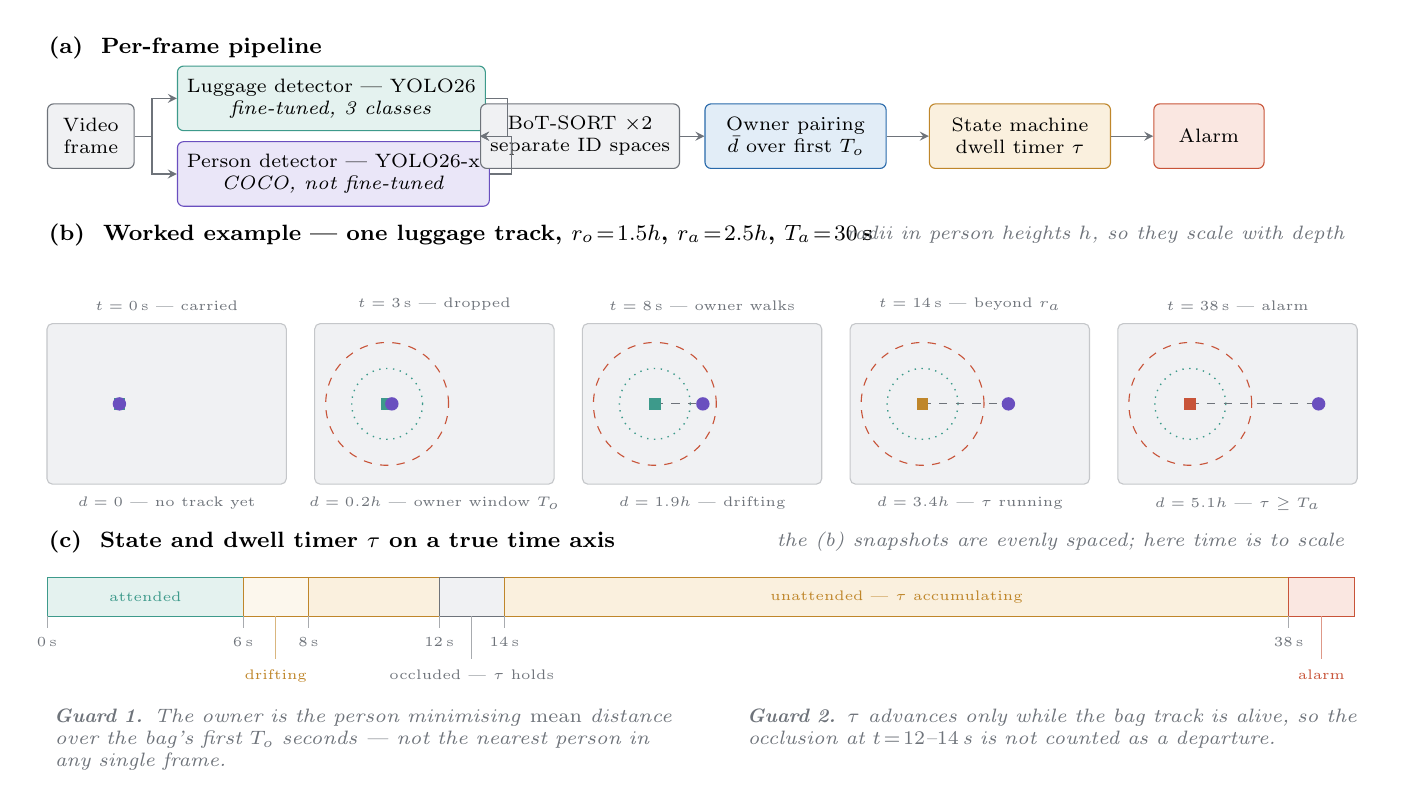
\begin{tikzpicture}[x=1cm,y=1cm]

%% ================= (a) pipeline =========================================
% Node widths are measured, not guessed: at \scriptsize the two detector
% boxes are 3.26 cm wide, so they must start far enough left of the tracker
% box that (dl.east) stays to the LEFT of (tr.west) -- otherwise the
% "-- ++(0.28,0) |- (tr.west)" connector doubles back on itself and draws a
% hook over the tracker box. Slots below are laid out with a 0.55 cm gap.
\node[font=\footnotesize\bfseries,anchor=west] at (0,2.22) {(a)~~Per-frame pipeline};

\node[blk,minimum width=11mm,anchor=west]  (fr) at (0.10,1.10) {Video\\frame};
\node[teal,minimum width=33mm,anchor=west] (dl) at (1.75,1.58) {Luggage detector \textemdash{} YOLO26\\\textit{fine-tuned, 3 classes}};
\node[purp,minimum width=33mm,anchor=west] (dp) at (1.75,0.62) {Person detector \textemdash{} YOLO26-x\\\textit{COCO, not fine-tuned}};
\node[blk,minimum width=23mm,anchor=west]  (tr) at (5.60,1.10) {BoT-SORT $\times2$\\separate ID spaces};
\node[blu,minimum width=23mm,anchor=west]  (op) at (8.45,1.10) {Owner pairing\\$\bar d$ over first $T_o$};
\node[amb,minimum width=23mm,anchor=west]  (sm) at (11.30,1.10) {State machine\\dwell timer $\tau$};
\node[cor,minimum width=14mm,anchor=west]  (al) at (14.15,1.10) {Alarm};

\draw[fl] (fr.east) -- ++(0.22,0) |- (dl.west);
\draw[fl] (fr.east) -- ++(0.22,0) |- (dp.west);
\draw[fl] (dl.east) -- ++(0.27,0) |- (tr.west);
\draw[fl] (dp.east) -- ++(0.27,0) |- (tr.west);
\draw[fl] (tr.east) -- (op.west);
\draw[fl] (op.east) -- (sm.west);
\draw[fl] (sm.east) -- (al.west);

%% ================= (b) worked example ===================================
\node[font=\footnotesize\bfseries,anchor=west] at (0,-0.15) {(b)~~Worked example \textemdash{} one luggage track, $r_o\!=\!1.5h$, $r_a\!=\!2.5h$, $T_a\!=\!30$\,s};
\node[lbl,anchor=east] at (16.70,-0.15) {radii in person heights $h$, so they scale with depth};

\def\sc#1#2#3#4#5#6{%
  \begin{scope}[shift={(#1,-2.30)}]
    \draw[draw=cGry!40,fill=cGryBg,rounded corners=2pt] (-1.52,-1.02) rectangle (1.52,1.02);
    \ifnum#6>0
      \draw[draw=cCor,dashed,line width=0.4pt] (-0.60,0) circle (0.78);
      \draw[draw=cTeal,dotted,line width=0.5pt] (-0.60,0) circle (0.45);
    \fi
    \ifnum#6>0 \draw[draw=cGry,line width=0.4pt,dashed] (-0.60,0) -- (#2,0); \fi
    \fill[#5] (-0.675,-0.075) rectangle (-0.525,0.075);
    \fill[cPurp] (#2,0) circle (0.085);
    \node[font=\tiny,text=cGry,anchor=south] at (0.0,1.06) {#3};
    \node[font=\tiny,text=cGry,anchor=north] at (0.0,-1.06) {#4};
  \end{scope}}

\sc{1.62}{-0.60}{$t=0$\,s \textemdash{} carried}{$d=0$ \textemdash{} no track yet}{cTeal}{0}
\sc{5.02}{-0.54}{$t=3$\,s \textemdash{} dropped}{$d=0.2h$ \textemdash{} owner window $T_o$}{cTeal}{1}
\sc{8.42}{0.01}{$t=8$\,s \textemdash{} owner walks}{$d=1.9h$ \textemdash{} drifting}{cTeal}{1}
\sc{11.82}{0.49}{$t=14$\,s \textemdash{} beyond $r_a$}{$d=3.4h$ \textemdash{} $\tau$ running}{cAmb}{1}
\sc{15.22}{1.03}{$t=38$\,s \textemdash{} alarm}{$d=5.1h$ \textemdash{} $\tau\ge T_a$}{cCor}{1}


%% ================= (c) timeline =========================================
% Time axis: x = 0.10 + 0.415*t, so 0 s -> 0.10, 6 -> 2.59, 8 -> 3.42,
% 12 -> 5.08, 14 -> 5.91, 38 -> 15.87, 40 -> 16.70.
% The bar is 0.50 cm tall (was 0.36) so the two inline labels sit clear of
% the rules, and ALL labels below it live on exactly two levels: timestamps
% at -5.16, segment names at -5.56. The vertical droplines that used to run
% down from the (b) snapshots are gone: the snapshots are evenly spaced but
% time is not, so those lines landed nowhere near their own timestamps.
\node[font=\footnotesize\bfseries,anchor=west] at (0,-4.05) {(c)~~State and dwell timer $\tau$ on a true time axis};
\node[lbl,anchor=east] at (16.70,-4.05) {the (b) snapshots are evenly spaced; here time is to scale};

\fill[cTealBg,draw=cTeal,line width=0.3pt]  (0.10,-5.00) rectangle (2.59,-4.50);
\fill[cAmbBg!55,draw=cAmb,line width=0.3pt] (2.59,-5.00) rectangle (3.42,-4.50);
\fill[cAmbBg,draw=cAmb,line width=0.3pt]    (3.42,-5.00) rectangle (5.08,-4.50);
\fill[cGryBg,draw=cGry,line width=0.3pt]    (5.08,-5.00) rectangle (5.91,-4.50);
\fill[cAmbBg,draw=cAmb,line width=0.3pt]    (5.91,-5.00) rectangle (15.87,-4.50);
\fill[cCorBg,draw=cCor,line width=0.3pt]    (15.87,-5.00) rectangle (16.70,-4.50);

\node[font=\tiny,text=cTeal] at (1.35,-4.75) {attended};
\node[font=\tiny,text=cAmb]  at (10.89,-4.75) {unattended \textemdash{} $\tau$ accumulating};

% level 1 -- timestamps, every event on one line
\foreach \x/\t in {0.10/0\,s, 2.59/6\,s, 3.42/8\,s, 5.08/12\,s, 5.91/14\,s, 15.87/38\,s}{
  \draw[draw=cGry!60,line width=0.3pt] (\x,-5.00) -- (\x,-5.14);
  \node[font=\tiny,text=cGry,anchor=north] at (\x,-5.14) {\t};}

% level 2 -- names of the segments too narrow to label inline
\draw[draw=cAmb!60,line width=0.3pt] (3.005,-5.00) -- (3.005,-5.54);
\node[font=\tiny,text=cAmb,anchor=north] at (3.005,-5.56) {drifting};
\draw[draw=cGry!60,line width=0.3pt] (5.495,-5.00) -- (5.495,-5.54);
\node[font=\tiny,text=cGry,anchor=north] at (5.495,-5.56) {occluded \textemdash{} $\tau$ holds};
\draw[draw=cCor!60,line width=0.3pt] (16.285,-5.00) -- (16.285,-5.54);
\node[font=\tiny,text=cCor,anchor=north] at (16.285,-5.56) {alarm};

%% ================= guards ==============================================
\node[lbl,anchor=north west,align=left,text width=79mm] at (0.10,-6.05)
 {\textbf{Guard 1.} The owner is the person minimising \emph{mean} distance over the
  bag's first $T_o$ seconds \textemdash{} not the nearest person in any single frame.};
\node[lbl,anchor=north west,align=left,text width=79mm] at (8.90,-6.05)
 {\textbf{Guard 2.} $\tau$ advances only while the bag track is alive, so the
  occlusion at $t\!=\!12$--$14$\,s is not counted as a departure.};

\end{tikzpicture}
\end{document}
